\chapter{Revisão Bibliográfica}
Neste Capítulo serão abordados alguns conceitos e técnicas, necessárias para
compreender o trabalho proposto, que é 
gerar malha e mapa de altura com tamanho pseudo-infinitos, de maneira procedural
e não assistida, suportando mais de um bioma.

\section{Biomas}
Existem mais que um conceito de bioma, um bastante adotado considera bioma como
uma área do espaço geográfico, representada por um tipo uniforme de ambiente, o
mesmo pode ser classificado de acordo com o macroclima, fitofisionomia (formação),
solo e a altitude, os elementos que maus caracterizam os ambientes continentais, 
este é o conceito de \cite{coutinho2006conceito}, usando como base descrições
de \cite{walter1986vegetaccao}.

Porém neste trabalho o conceito de bioma vai ser outro, o resultado deste
vai ser unicamente mapas de altura, então a única característica que é relevante
são as altitudes do solo e seus padrões, descartando dados como tipo da
vegetação e sua distribuição, umidade e entre outros. Então no restante 
do trabalho, quando for usado os termos "característica do bioma", o mesmo vai
se referir a alguma característica de altitude do bioma.

Para fins de restringir o escopo do projeto vamos agrupar os biomas por padrões
de relevo e não por fauna e flora como feito no conceito apresentado acima,
estes biomas serão: cordilheiras (cadeias de montanha), planícies.

Como este trabalho é voltado para a área de jogos, dentro da comunidade de jogadores
é bem aceito usar o termo bioma de forma mais genérica, o jogo Minecraft usa o
termo e entre seus biomas se encontra \textit{Extreme Hills} e \textit{Plains}.

\section{Representação das Regiões}
Neste trabalho serão implementadas três maneiras de representar a malha de
regiões, malha de quadrados, malha triangular e diagrama de Voronoi.

Um bioma vai pertencer a um conjunto de regiões, na imagem \ref{fig:squadStripBiomes}
que usa uma malha de quadrados, onde os segmentos de retas vermelhas são fronteiras entre
biomas.
\begin{figure}[H]
    \centering
    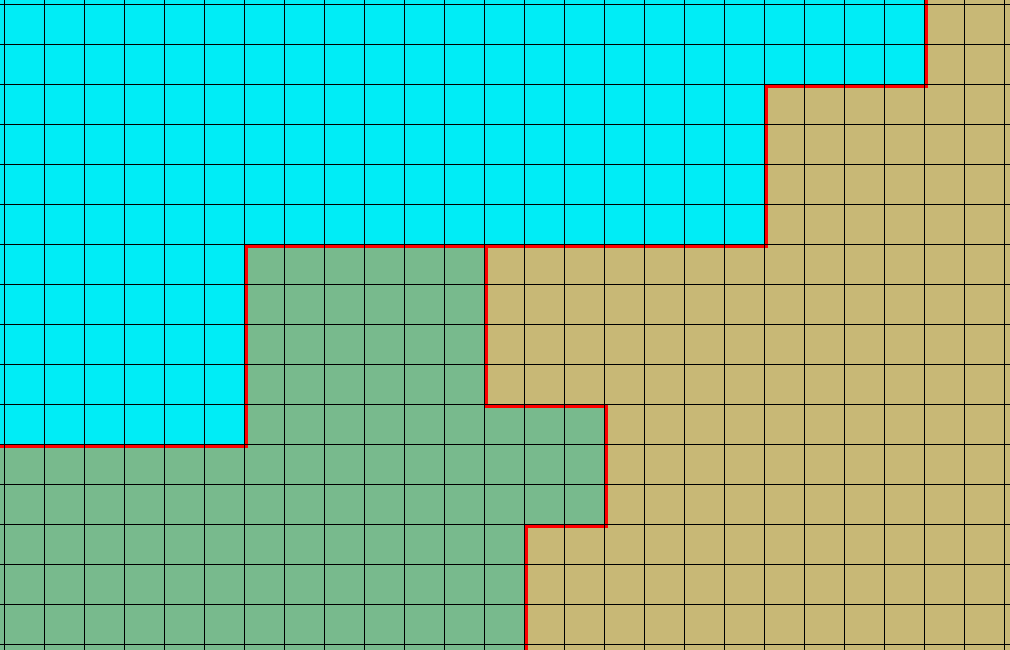
\includegraphics[width=0.7\textwidth]{figuras/squadStripBiomes.png}
    \caption{Malha de quadrados com divisão de biomas}
    \label{fig:squadStripBiomes}
\end{figure}
\subsection{Malhas de quadrado}
Este modelo já apresentado na figura \ref{fig:squadStripBiomes}, nele cada
quadrado é uma região, os vértices armazenados se encontram nos quatro cantos
do quadrado, então um vértice é comum a quatro quadrados, cada um deles
compartilhando o vértice com os quadrados adjacentes, as arestas entre vértices
vizinhos são uma fronteira entre regiões, e tem a possibilidade desta aresta ser
também uma fronteira entre biomas.

Devido ao padrão podemos perceber que não temos a necessidade de armazenar arestas
em memória, já que a mesma só vai existir entre vértices vizinhos, o vértice
$v_{i j}$ tem como vizinhos o conjunto $\{v_{i+1 j}, v_{i-1 j}, v_{i j+1}, v_{i j-1}\}$.
\subsection{Malha triangular}
Usando a mesma base de vértice da malha de quadrados, agora temos uma aresta
adicional, uma diagonal em cada quadrado do modelo anterior, dividindo a região
em duas, cada triangulo sendo uma região, como podemos ver na figura \ref{fig:vbo}.
Agora além do conjunto de arestas do modelo anterior, o vértice $v_{i j}$ também tem
aresta para os vértices $\{v_{i+1 j+1}, v_{i-1 j-1}\}$
\begin{figure}[H]
    \centering
    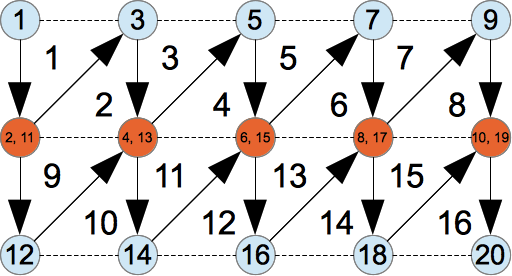
\includegraphics[width=0.5\textwidth]{figuras/vbo.png}
    \caption{Malhas de triângulos, retirado de \cite{androidtrianglestrip}}
    \label{fig:vbo}
\end{figure}


\subsection{Diagrama de Voronoi}
Um diagrama de Voronoi é uma partição no plano para separar regiões, recebendo
como entrada um conjunto de pontos chamados de \textit{sites}, o algoritmo
separa as regiões de cada \textit{site} deixando a fronteira equidistante entre eles
\cite{fortune1987sweepline}.

Como está implementação vai ser não assistida estes sites precisam ser colocados
aleatoriamente e proceduralmente, para não ocorrer aglomerações de site, já
que existe a possibilidade de acontecer na geração de \textit{sites} aleatórios,
será usado o algoritmo de Lloyd's para relaxar os sites, o conjunto dessas
técnicas já foi usado por \cite{patel2010polygonal}, para gerar malha de regiões,
segue uma imagem de seu diagrama na figura \ref{fig:voronoi-2-lloyd}, este diagrama
foi usado para alcançar o resultado já mostrado na ilustração \ref{fig:voronoi-map-goal-distorted}.
\begin{figure}[H]
    \centering
    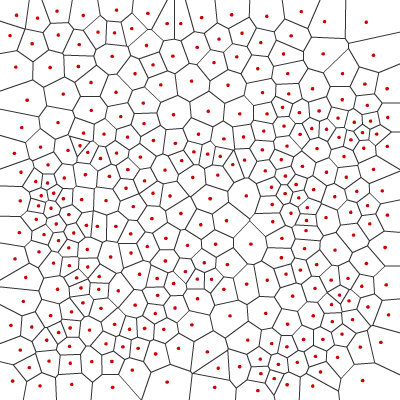
\includegraphics[width=0.5\textwidth]{figuras/voronoi-2-lloyd.png}
    \caption{Diagrama de Voronoi com algoritmo de Lloyd's aplicado, por \cite{patel2010polygonal}}
    \label{fig:voronoi-2-lloyd}
\end{figure}

\section{Ruído de Perlin}
Bons geradores de números aleatórios geram números onde não existe relação entre
eles, porem se montado um gráfico com eles, o resultado não teria um aspecto
orgânico, então para o terreno ter um relevo mais parecido com o encontrado na 
natureza é usado uma função de ruído \cite{shiffman2012nature}, está comparação
pode ser feita com a imagem \ref{fig:randomAndNoise}. 
\begin{figure}[H]
    \centering
    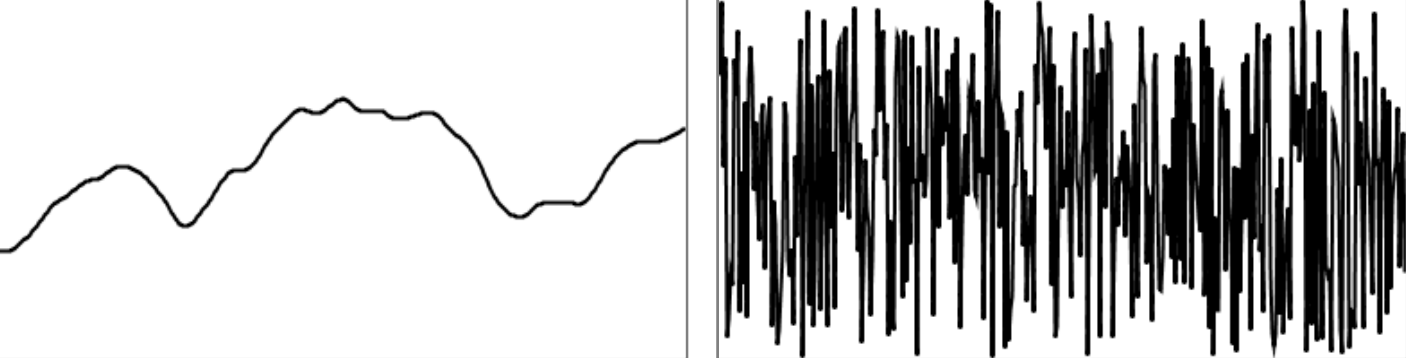
\includegraphics[width=0.7\textwidth]{figuras/randomAndNoise.png}
    \caption{Da esquerda, função de ruído, função de pontos aleatórios. Por \cite{shiffman2012nature}}
    \label{fig:randomAndNoise}
\end{figure}

Uma função de ruído recebe como parâmetro as coordenadas em um espaço de $n$ dimensões,
retorna um valor entre $0$ e $1$ para tal posição\cite{shiffman2012nature}.

Na figura \ref{fig:randomAndNoise} vimos o ruído unidimensional, o ruído
tem a complexidade $O(2^n)$, sendo $n$ a quantidade de dimensões \cite{zucker2001perlin}.
Este mesmo ruído unidimensional pode ser usado nas fronteiras entre biomas, dando
um aspecto mais natural á fronteiras, da mesma maneira que foi usado nas bordas
das ilhas no trabalho de \cite{patel2010polygonal}. Contudo, para gerar altura
em um cenário tridimensional precisamos usar o ruído bidimensional, existem
implementações do ruído em placas gráficas que calculam a função de ruído para 
$\{1, 2, 3\}$ dimensões em único ciclo \cite{perlin2002improving}.

No ruído unidimensional a resposta é uma interpolação entre seus vizinhos, que
neste caso são apenas $2$, caso o parâmetro do ruído for $x_{i}$, o mesmo só tem 
como vizinhos, $x_{i+1}$ e $x_{i-1}$, quando a dimensão aumenta e por conta disso
os parâmetros também, a quantidade de vizinhos também aumenta \cite{shiffman2012nature}, 
como o mesmo exemplifica na ilustração \ref{fig:1dto2dnoise}.
\begin{figure}[H]
    \centering
    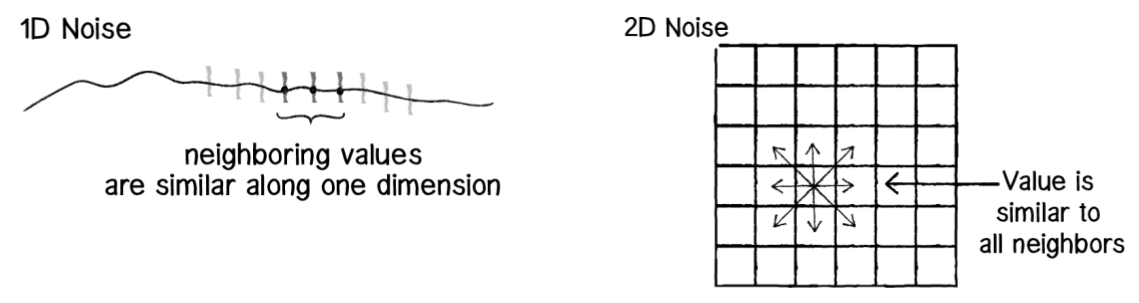
\includegraphics[width=0.7\textwidth]{figuras/1dto2dnoise.png}
    \caption{Vizinhas para função de ruído, $1d$ para $2d$. Por \cite{shiffman2012nature}}
    \label{fig:1dto2dnoise}
\end{figure}

O ruído de Perlin usa a função ruído explicada acima várias vezes, cada uma é chamada
de oitava, cada oitava usa amplitude e frequência diferente, a quantidade de oitavas
usada varia de implementações para necessidades, a primeira oitava é gerada com uma
amplitude alta e frequência baixa, as próxima oitava tem a metade da amplitude e 
o dobro da frequência, o ruído de Perlin é a soma de todas as oitavas computadas,
adaptado de Hugo Elias \cite{carli2012canion} gerou as imagens
\ref{fig:perlin1d} e \ref{fig:perlin2d} do ruído de Perlin em uma e duas
dimensões respectivamente.
\begin{figure}[H]
    \centering
    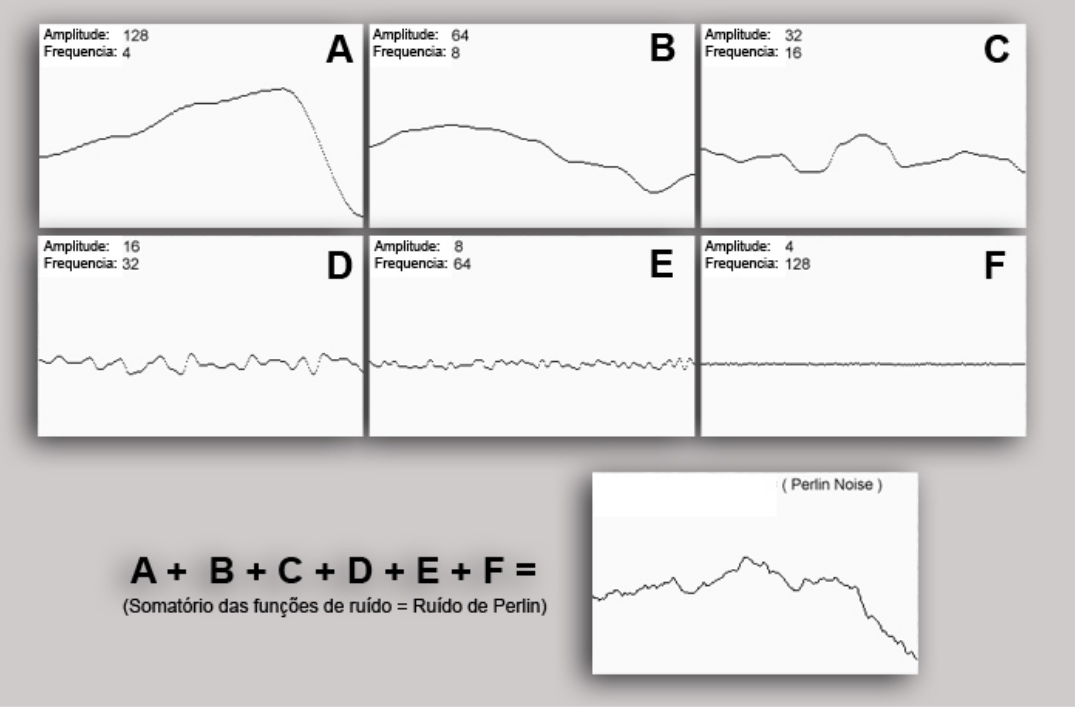
\includegraphics[width=0.7\textwidth]{figuras/perlin1d.png}
    \caption{Gerando ruído de Perlin para uma dimensão}
    \label{fig:perlin1d}
\end{figure}
\begin{figure}[H]
    \centering
    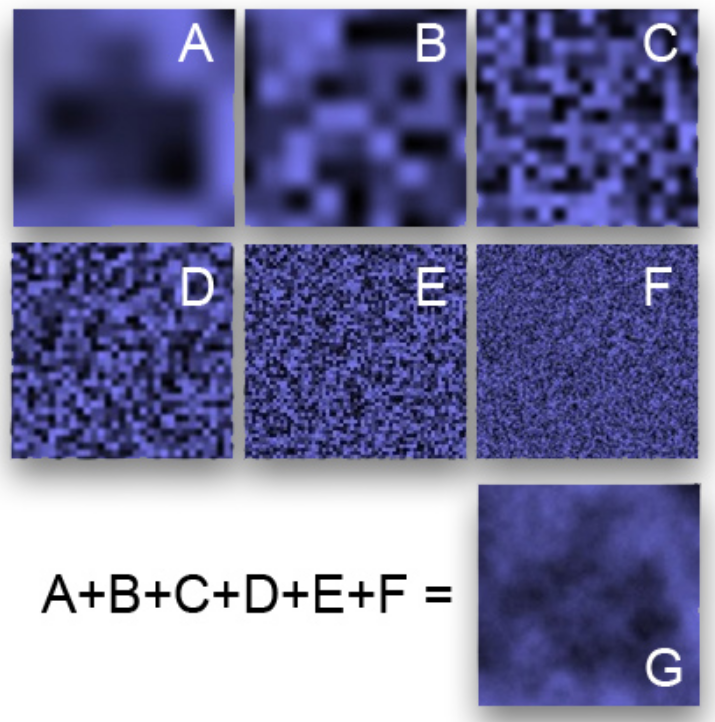
\includegraphics[width=0.6\textwidth]{figuras/perlin2d.png}
    \caption{Gerando ruído de Perlin para duas dimensões}
    \label{fig:perlin2d}
\end{figure}

\section{Mapas de Altura}
Mapas de altura é uma maneira de representar altitudes de um terreno, e essa
será uma das saídas desta implementação proposta, mapas de altura costumam ser, imagens
onde os pontos mais claros representam pontos mais elevados e os escuros regiões mais baixas.
A imagem \ref{fig:perlin2d} já traz exemplos de mapas de altura.

Um mapa de altura pode ser usado para ser renderizado em diferentes perspectivas,
ou usar processos que geram imagens de luz e sombra, ilustrados na figura \ref{fig:hmap} de \cite{dachsbacher2006interactive}.
\begin{figure}[H]
    \centering
    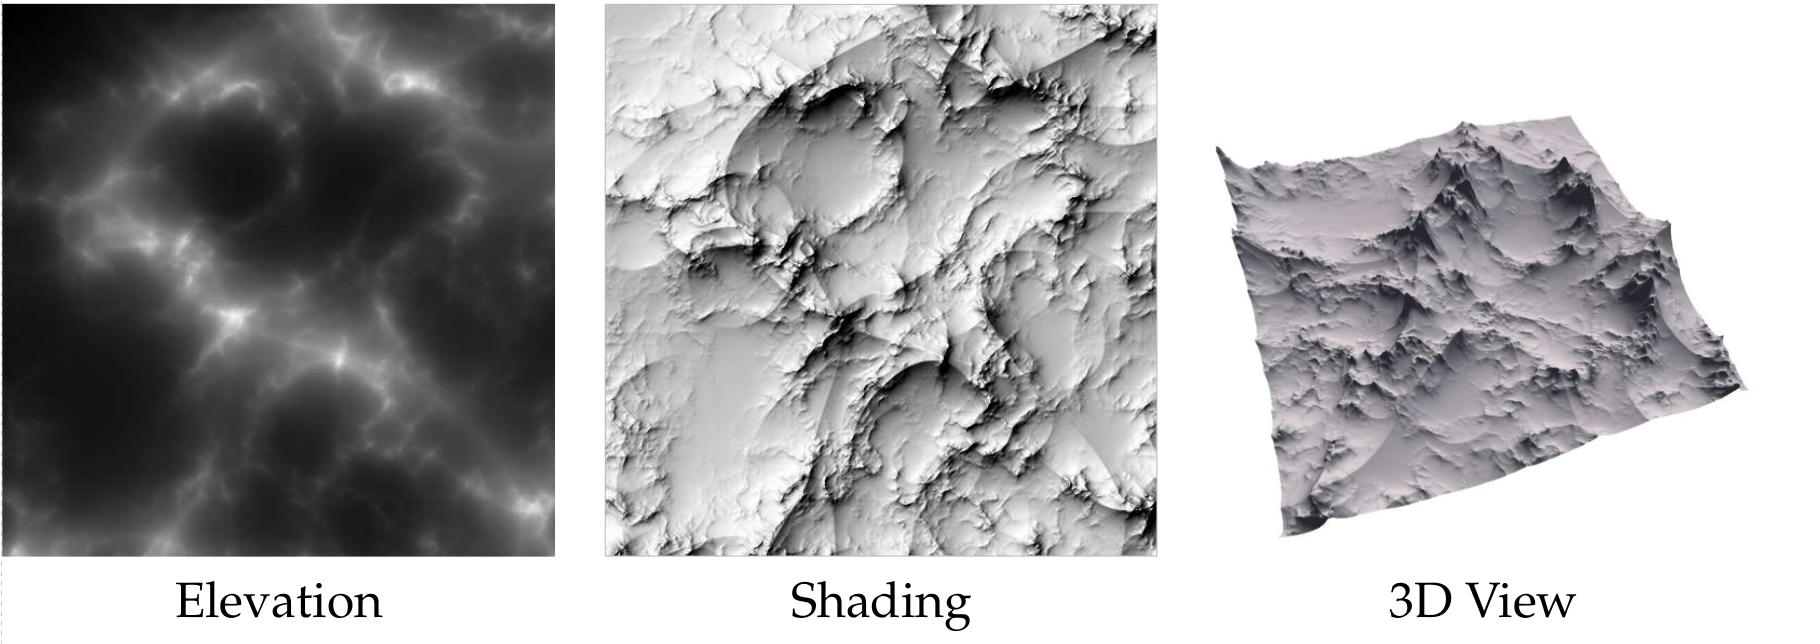
\includegraphics[width=0.75\textwidth]{figuras/hmap.png}
    \caption{Diferentes maneiras de usar um mapa de altura por }
    \label{fig:hmap}
\end{figure}


\section{Trabalho de Carli}
O trabalho do \cite{carli2012canion}, não só gera o mapa de altura, mas também
faz busca de percursos de rio e agentes no mapa. As maiores semelhanças deste 
trabalho com o proposto, é que faz uso da manipulação dos resultados do ruído de
de Perlin para recriar alguns padrões de relevo e também é uma técnica não assistida,
entretanto no projeto que 
estou propondo se faz necessário ter pelo menos duas manipulações de ruído distintas
e criar fronteiras contínuas quando as mesmas se encontram. O resultado final de
\cite{carli2012canion} já foi apresentado na introdução.
